% Exam Template for University of Management and Technology Lahore
% Author: Abu Bakar Siddique
% The folder of this tex should also contains UMTLogo.jpg and exam.cls
%
% Adapted From:
% Exam Template for UMTYMP and Math Department courses
% Using Philip Hirschhorn's exam.cls: http://www-math.mit.edu/~psh/#ExamCls
%
% run pdflatex on a finished exam at least three times to do the grading table on front page.
%
%%%%%%%%%%%%%%%%%%%%%%%%%%%%%%%%%%%%%%%%%%%%%%%%%%%%%%%%%%%%%%%%%%%%%%%%%%%%%%%%%%%%%%%%%%%%%%

\documentclass[11pt]{exam}
\RequirePackage{amssymb, amsfonts, amsmath, latexsym, verbatim, xspace, setspace}
\RequirePackage{tikz, pgflibraryplotmarks}
\usetikzlibrary{shapes.geometric,arrows,fit,matrix,positioning}
\tikzset
{
    treenode/.style = {circle, draw=black, align=center,
                          minimum size=1cm, anchor=center},
}
\usepackage[none]{hyphenat}
\usepackage[margin=1in]{geometry}
\usepackage{multirow}
\usepackage{lipsum,hyperref}

%%%%%%%%%%%%%%%%%%%%%%%%%%%%%%%%%%%%%%%%%%%%%%%%%%%%%%%%%%%%%%%%%%%%%%%%%%%%%%%%%%%%%
%            E X A M   I N F O R M A T I O N
%%%%%%%%%%%%%%%%%%%%%%%%%%%%%%%%%%%%%%%%%%%%%%%%%%%%%%%%%%%%%%%%%%%%%%%%%%%%%%%%%%%%%

\newcommand{\courseCode}{EE210}
\newcommand{\courseTitle}{Data Structures And Algorithms}
\newcommand{\examDate}{April 09, 2013}
\newcommand{\examType}{Mid Term}
\newcommand{\RP}{Mr. Saleem Ata (Sec A \& E), Abu Bakar Siddique (Sec  B, C \& D)}
\newcommand{\semester}{Spring 2013}
\newcommand{\academicYear}{2013}
\newcommand{\timeAllowed}{30 Minutes}
\newcommand{\totalMarks}{15}

\newcommand{\rowSpace}{1.2ex}

\singlespacing
% \onehalfspacing
% \doublespacing
% For an exam, single spacing is most appropriate

% For an exam, we generally want to turn off paragraph indentation
%\parindent 3ex

\title{\vspace{-7ex} University of Management \& Technology\vspace{-1ex}}
\author{Department of Electrical Engineering
}
\date{}

\begin{document} 

\begin{center}

\includegraphics[width=2in]{pku}
\\[.5em]\LARGE\bfseries Department of Philosophy
\end{center}

%-----------------------------------------------
%        Header
%-----------------------------------------------
\vspace{2em}
\pagestyle{headandfoot}
\firstpageheader{}{}{}
\runningheader{ \textbf{Student ID:}}{}{\textbf{Section:}\quad}
\runningheadrule
\runningfooter{}{Page \thepage\ of \numpages}{}

\begin{flushright}
\begin{tabular}{p{1.5in} p{2in} p{.05in} p{1.2in} p{1in}}

\textbf{Student ID}&\hrule && \textbf{Section} & \hrule \\ [\rowSpace]
\textbf{Student Name}&\hrule && \textbf{Semester}& \semester\\ [\rowSpace]
\textbf{Student Signature}&\hrule&&&\\ [\rowSpace]
\textbf{Course Code}&\courseCode && \textbf{Academic Year} & \academicYear\\
\textbf{Course Title}& \courseTitle && \textbf{Time Allowed} & \timeAllowed\\
\textbf{Exam Date}& \examDate && \textbf{Total Marks}& \totalMarks\\
\textbf{Exam}& \examType && & \\
\textbf{Resource Person(s)} & \multicolumn{4}{p{4.5in}}{\RP}\\
\end{tabular}
\end{flushright}

\noindent\rule{\textwidth}{1pt}
\small
\begin{center}
\textbf{DO  NOT  OPEN  THIS  EXAM  UNTIL  TOLD  TO  DO  SO}
\end{center}
The instructions below must be followed strictly. Failure to do so can result in serious grade loss. You must
\begin{itemize}
  \item Keep your eyes on your own paper.
  \item Switch off your mobile phones completely.
\end{itemize}
\begin{center}
\textbf{SPECIFIC INSTRUCTIONS}
\end{center}
\begin{itemize}
\item \textbf{Calculator Allowed, Closed Book, Closed Notes.}
\item \textbf{No extra sheet} will be given. Use the available space wisely.
\item \textbf{Use a blue or black} ball point or pen. Please do not use lead pencils.
\item \textbf{Provide final answers} in the space provided.You may use back blank sheets for rough work.
\end{itemize}
\noindent\rule{\textwidth}{1pt}

\begin{center}
\textbf{Certificate to be filled at the time of exam}
\end{center}

I have counted all \numpages\ pages in this exam and no page is missing. \hfill \textbf{Student Signature}

\begin{center}
\vspace{0pt}
\cellwidth{3em}
\gradetablestretch{1}
\vqword{Questions}
\addpoints % required here by exam.cls, even though questions haven't started yet.
\gradetable[h][questions]%[pages]  % Use [pages] to have grading table by page instead of question

%\pointtable[h][questions]
%\end{minipage}
\end{center}

\begin{center}
\textbf{Certificate to be filled during paper viewing}
\end{center}

I have reviewed my paper and all \numquestions\ questions have been marked with\\ no
 part left unmarked. Counting is also correct. \hfill \textbf{Student Signature}

\newpage % End of cover page

%%%%%%%%%%%%%%%%%%%%%%%%%%%%%%%%%%%%%%%%%%%%%%%%%%%%%%%%%%%%%%%%%%%%%%%%%%%%%%%%%%%%%
%            Q U E S T I O N S
%
% See http://www-math.mit.edu/~psh/#ExamCls for full documentation, but the questions
% below give an idea of how to write questions [with parts] and have the points
% tracked automatically on the cover page.
%%%%%%%%%%%%%%%%%%%%%%%%%%%%%%%%%%%%%%%%%%%%%%%%%%%%%%%%%%%%%%%%%%%%%%%%%%%%%%%%%%%%%

\begin{questions}

% Basic question
%\addpoints
%\question[10] Differentiate $f(x)=x^2$ with respect to $x$.

\addpoints
\question[3] Write Pre-Order, In-Order and Post-Order traversals of following tree:
\begin{center}
    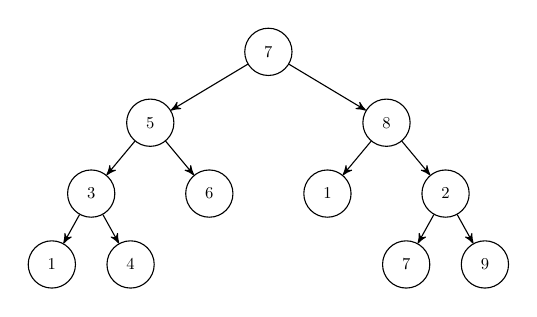
\begin{tikzpicture}[->,>=stealth',level/.style={sibling distance = 5cm/#1,
    level distance = 1.5cm},scale=0.6, transform shape]

    \node [treenode] {7}
    child{
        node [treenode] {5}
        child{
            node [treenode] {3}
            child{ node [treenode] {1} }
            child{ node [treenode] {4} }
        }
        child{ node [treenode] {6} }
    }
    child{
        node [treenode] {8}
        child{
        	node [treenode] {1}
        }
        child{
            node [treenode] {2}
            child{ node [treenode] {7} }
            child{ node [treenode] {9} }
        }
    }
;
    \end{tikzpicture}
\end{center}
\vspace{4in}

\addpoints
\question[2] A Binary Tree has 37 nodes. What is the minimum height of the tree that can take all of these nodes? Take height of a single node tree as 1.
\vspace{3in}

	\href{https://tex.stackexchange.com/questions/782/what-are-the-available-documentclass-types-and-their-uses}{{What are the available ``documentclass" types and their uses?}}

\addpoints
\question[3] Make structure of a binary tree that has following Pre-Order and In-Order traversals:
\begin{description}
\item[Pre-Order:] A, B, D, E, F, G, C
\item[In-Order:] D, B, F, E, G, A, C
\end{description}
\vspace{6in}

\addpoints
\question[1] How many comparisons would take place when finding a value in a sorted list of 1024 entries using binary search algorithm? (2 Marks)
\vspace{2in}

\addpoints
\question[4] Construct binary search tree when values are inserted in following order:\\
 $\longrightarrow$ 9, 13, 12, 1, 7, 25, 4, 19, 3, 23, 11, 4, 27,6
\newpage

\addpoints
\question[2] Starting with empty stack, what would be the contents of the stack after following operations are performed.Draw the stack after the following operations
\begin{itemize}
\item Push(56)
\item Push(92)
\item Push(7)
\item Pop()
\item Push(5)
\item Pop()
\end{itemize}

\vspace{4in}

\end{questions}
\end{document}
